\graphicspath{{content/1_literatureReview/figures/}}
\section{Operational Amplifiers}

\subsection{Basic Principles}
An operational amplifier or "op-amp" is a type of differential amplifier. Fundamentally, these amplifiers multiply the difference between the voltages
at their positive ($V^+$) and negative ($V^-$) terminals by a specified gain factor. This gain, $A_d$, is also known as the \textit{differential-mode gain}.
Although differential amplifiers are often designed for a specific $A_d$, op-amps usually aim to
have as high a differential gain as possible (for an ideal op-amp, $A_d \to \infty$).

$A_d$ is also known as the \textit{open-loop gain}. Due to a large-valued open-loop gain, op-amps are often used in \textit{closed-loop} configurations, which are more flexible
and take advantage of this large $A_d$. These configurations arise when there is a negative feedback loop from the output which is connected to the negative input terminal.

\subsection{Limitations}
Often, it is applicable to design an amplifier circuit using the ideal operational amplifier model. This model assumes no current into the input terminals, an infinite, linear,
differential-mode gain, and that terminal voltage $V^+ = V^-$ when negative feedback is present. This model, however, may be inadequate
in low voltage, high current or high frequency environments. The following are common limitations of non-ideal op-amps \cite{opAmpLimitations}:
\begin{itemize}
    \item Voltage supply saturation. For given k, output cannot go above $V_{ss} - k$ or below  $V_{dd} + k$.
    \item Finite bandwidth. Output signal magnitude reduces at high frequencies. This effect can be analysed using the gain-bandwidth product (GBWP) equation.
    \item Offset voltage/bias current. Even with no input, there exists a small "offset voltage" and "bias current" into the amplifier.
          This results in unwanted voltage at the output.
    \item Finite slew rate. The output cannot change quicker than a specified rate. This is different to the finite bandwidth limitation, but has a similar limiting effect.
    \item Finite common-mode rejection ratio (CMRR). An op-amp should ideally only amplify $V_{+} - V_{-}$, but also amplifies the unwanted common signal (e.g. noise) on both inputs.
\end{itemize}

\subsection{Key Specifications}
Based around the above limitations, op-amp datasheets provide a number of key specifications that may be important for design.
The op-amp used in this project is the MCP6242. Listed below are its notable specifications \cite{datasheetMCP6242}:
\begin{itemize}
    \item Typical CMMR of 75 dB (DC) to 65 dB (1 kHz).
    \item Ability to output between 0.035 and 5.465 V if $V_{ss}$ = 5.5 V and $V_{dd}$ = 0 V.
    \item Slew rate of 0.3 V/uS.
    \item Common mode input range from $V_{dd} - \SI{0.3}{V}$ to $V_{ss} + \SI{0.3}{V}$.
    \item Maximum current output of $\SI{23}{mA}$.
    \item Gain-bandwidth product of $\SI{550}{kHz}$.
\end{itemize}

\subsection{Configurations}
A number of well-known op-amp configurations exist that all achieve slightly different amplification goals. The following list compares some common configurations [3].
Although certain circuits have two inputs, one of the inputs can be set to a specific voltage level for to add an offset to the output. These configurations can also
be expanded to allow for signal "summing" by simply adding more inputs in parallel.


\begin{center}

    \begin{tabular}{|p{3.5cm}|p{6cm}|p{6cm}|}
        \hline
        Type            & Advantages
                               & Disadvantages                               \\
        \hline
        Non-inverting   & - Simple to design and build                    & - Large input bias currents                 \\
                        & - High input impedance                          & - Amplifies noise from input                \\
        \hline
        Differential    & - Good noise rejection                          & - Complex design                            \\
                        & - Flexible                                      & - Low input impedance                       \\
        \hline
        Instrumentation & - Same as differential                          & - Complex and expensive design              \\
                        & - Very high input impedance                     &                                             \\
        \hline
    \end{tabular}
\end{center}

\begin{figure}[!h]
    \centering
    \begin{minipage}{.23\textwidth}
        \centering
        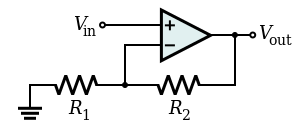
\includegraphics[width=.8\linewidth]{opAmp_nonInverting}
        \captionof{figure}{Non-Inverting Amplifier \cite{opAmpConfigurations}}
        \label{fig:opamp-non-inverting}
    \end{minipage}
    \begin{minipage}{.23\textwidth}
        \centering
        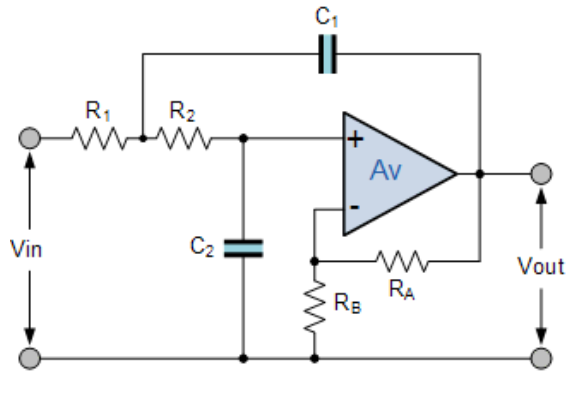
\includegraphics[width=0.8\linewidth]{opAmp_nonInverting_modified}
        \captionof{figure}{Modified Non-Inverting Amplifier \cite{opAmpSecondOrderFilters}}
        \label{fig:opamp-non-inverting-filter}
    \end{minipage}        
    \begin{minipage}{.23\textwidth}
        \centering
        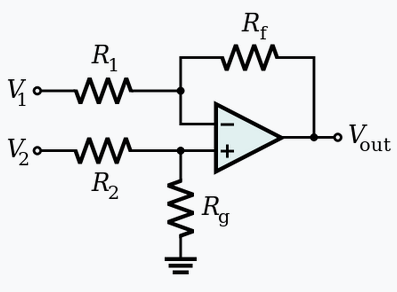
\includegraphics[width=.8\linewidth]{opAmp_differential}
        \captionof{figure}{Differential Amplifier \cite{opAmpConfigurations}}
        \label{fig:opamp-differential}
    \end{minipage}
    \begin{minipage}{.23\textwidth}
        \centering
        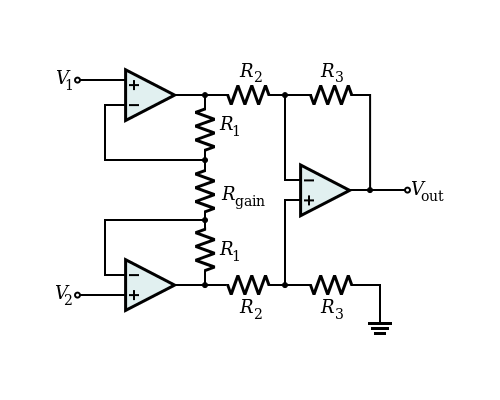
\includegraphics[width=0.9\linewidth]{opAmp_instrumentation}
        \captionof{figure}{Instrumentation Amplifier \cite{opAmpConfigurations}}
        \label{fig:opamp-instrumentation}
    \end{minipage}

\end{figure}

\pagebreak